\documentclass{article}
\usepackage{listings}
\usepackage{color}
\usepackage{float}
\usepackage{graphicx}

\definecolor{dkgreen}{rgb}{0,0.6,0}
\definecolor{gray}{rgb}{0.5,0.5,0.5}
\definecolor{mauve}{rgb}{0.58,0,0.82}

\lstset{
	frame=single,
	language=C,
	belowskip=3mm,
	showstringspaces=false,
	columns=flexible,
	captionpos=b,
	basicstyle={\small\ttfamily},
	numbers=left,
	numbersep=5pt,
	%numbers=none,
	numberstyle=\tiny\color{gray},
	keywordstyle=\color{blue},
	commentstyle=\color{dkgreen},
	stringstyle=\color{mauve},
	breaklines=true,
	breakatwhitespace=true,
	tabsize=4
}

\input kvmacros
\sloppy
\begin{document}

\title{Project 2A: Kernel Module Programming}
\author{\textit{Yesheng Ma}}
\date{\today}
{\bf\small CS353: Linux Kernel}\hfill{\bf\small 2017 Spring}
{\let\newpage\relax\maketitle}
\maketitle


\begin{abstract} 
In this project, we are going to write some Linux kernel modules. Kernel modules are code that can be dynamically loaded into the kernel at runtime. In particular, we will write three kernel modules that can output some info, accepts parameters, and create a proc file.
\end{abstract}


\section{Introduction to Kernel Modules}
A Linux kernel module is an object file that contains code to extend the running kernel. It is frequently used by kernel hackers to write programs that interacts with Linux kernel. Kernel module code runs in kernel mode. Some frequently used Linux commands related to kernel module include \verb|insmod|, \verb|rmmod|, and \verb|modinfo|.

Also, we need to get some idea about the Linux \verb|/proc| filesystem. \verb|/proc| is a \emph{virtual} file system, which is intended to expose some Linux kernel information to user. Also, we can configure the kernel using the \verb|/proc| filesystem.


\section{Build a Linux Kernel Module}
As we can checkout in the Linux kernel documentation project, there is a typical kind of Makefile script to build a Linux kernel as listed below.
\begin{lstlisting}
obj-m := homework1.o homework2.o homework3.o
KDIR := /lib/modules/$(shell uname -r)/build
PWD := $(shell pwd)

all:
	make -C $(KDIR) M=$(PWD) modules
clean:
	rm -f *.o *.ko *.mod.c Module.symvers modules.order
\end{lstlisting}
As we can see in the script, there is a special kind of Makefile object called \texttt{obj-m} and we need to specify the location of Linux header so that the kernel module can be successfully compiled.

\begin{figure}[H]
\centering
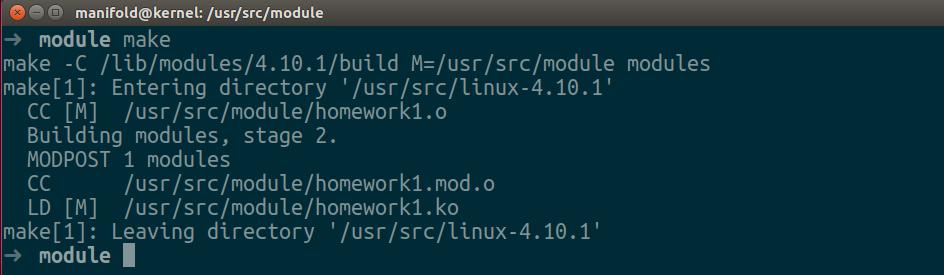
\includegraphics[width=10cm]{makehw1.png}
\caption{Building a Linux kernel module}
\end{figure}

\section{Core Implementation}
\subsection{Problem 1}
In this problem, we need to write a Linux kernel module that can print message to kernel buffer when it is loaded and cleaned up. The code snippet is shown as follows:
\begin{lstlisting}[language=c,caption=Module that output info on installation and exit]
#include <linux/module.h>
#include <linux/kernel.h>
#include <linux/init.h>

static int __init homework1_init(void) {
    printk(KERN_INFO "Hello world!\n");
    return 0;
}

static void __exit homework1_exit(void) {
    printk(KERN_INFO "Goodbye world!\n");
}

module_init(homework1_init);
module_exit(homework1_exit);
\end{lstlisting}

This program mainly includes three parts:
\begin{enumerate}
\item header file: these are Linux kernel headers which include necessary information to get kernel module compiled.
\item implementation code: the most important part is the definition of the \texttt{init} and \texttt{exit} functions, which uses the kernel function \texttt{printk} to print messages to kernel log buffer.
\item registration macro: the last two lines of this file registers the init and exit functions to the kernel module.
\end{enumerate}

As we can see in the following figure illustrating the result of running the kernel module. We can use the command \texttt{modinfo} to get information about this kernel module.
Then we install and remove the module and we can check the last two lines of the kernel log message using \texttt{dmesg | tail -n 2}.

\begin{figure}[H]
\centering
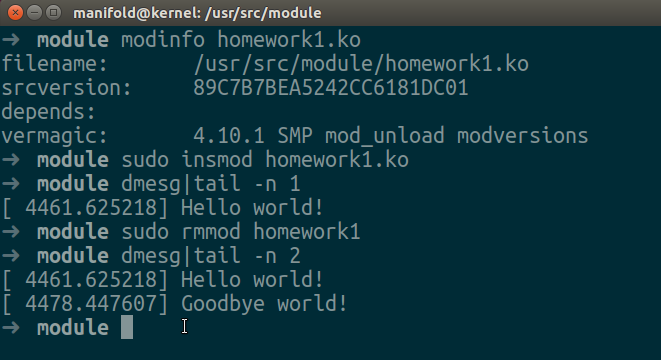
\includegraphics[width=11cm]{hw1res.png}
\caption{Result of homework 1}
\end{figure}

\subsection{Problem 2}
In this problem, we need to write a Linux kernel module that accepts a parameter of type int. We can easily use the kernel macro \texttt{module\_param} to declare a parameter of the module.
\begin{lstlisting}[language=c,caption=Module that takes an integer parameter]
#include <linux/kernel.h>
#include <linux/module.h>
#include <linux/init.h>
#include <linux/moduleparam.h>

MODULE_LICENSE("GPL");
MODULE_DESCRIPTION("Homework2");
MODULE_AUTHOR("Yesheng Ma");

static int test;
module_param(test, int, 0644);

static int __init homework2_init(void) {
    printk(KERN_INFO "Hello world!\n");
    printk(KERN_INFO "Params: test: %d\n", test);
    return 0;
}
static void __exit homework2_exit(void) {
    printk(KERN_INFO "Goodbye world!\n");
}

module_init(homework2_init);
module_exit(homework2_exit);
\end{lstlisting}

We can see that the code is nearly the same as the former one except that it can use the parameter \texttt{test} as if it is predefined. The result is shown as follows:
\begin{figure}[H]
\centering
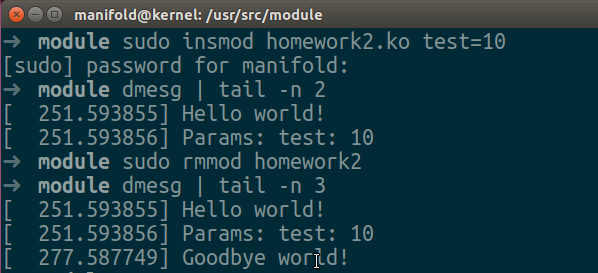
\includegraphics[width=11cm]{hw2res.png}
\caption{Result of homework 2}
\end{figure}

\subsection{Problem 3}
In this problem, we need to create a readable file in the \texttt{/proc} file system. I think this is the most challenging problem since the API for creating kernel module has largely changed and most documents online are quite deprecated. After referring to many documentations, I finally managed to finish this project.

As we can see in the following code, the most significant difference between Linux kernel version 2.6 and 4.10 is that we no longer have the function \verb|create_proc_entry|, on the other hand, we have \verb|proc_create|. The last parameter of this function is a file handle which defines how we can operate on a file. Also, the 4.10 kernel allows us to operate on a proc file as if this is a normal file. Thus we can use the API defined for one special kind of file \texttt{seq\_file} with related file oprations \verb|seq_printf|, \verb|single_open|. After we are done with the proc file, we can remove it by \verb|remove_proc_entry|.
\begin{lstlisting}[language=c,caption=Module to create a readable proc file]
#include <linux/module.h>
#include <linux/init.h>
#include <linux/kernel.h>

#include <linux/proc_fs.h>
#include <linux/seq_file.h>


MODULE_LICENSE("GPL");
MODULE_DESCRIPTION("homework3");
MODULE_AUTHOR("Yesheng Ma");

static int proc_show(struct seq_file *m, void *v) {
    seq_printf(m, "Message from a Linux kernel module.\n");
    return 0;
}

static int proc_open(struct inode *inode, struct file *file) {
    return single_open(file, proc_show, NULL);
}

static const struct file_operations fops = {
    .owner = THIS_MODULE,
    .open  = proc_open,
    .read  = seq_read,
    .llseek = seq_lseek,
    .release = single_release,
};

static int __init homework3_init(void) {
    struct proc_dir_entry *entry;
    entry = proc_create("homework3", 0, NULL, &fops);
    if (!entry) {
        return -ENOMEM;
    } else {
        printk(KERN_INFO "Proc_read_entry created successfully.\n");
        return 0;
    }
}

static void __exit homework3_exit(void) {
    remove_proc_entry("homework3", NULL);
    printk(KERN_INFO "Goodbye!\n");
}

module_init(homework3_init);
module_exit(homework3_exit);
\end{lstlisting}

The result of homework 3 is shown as follows:
\begin{figure}[H]
\centering
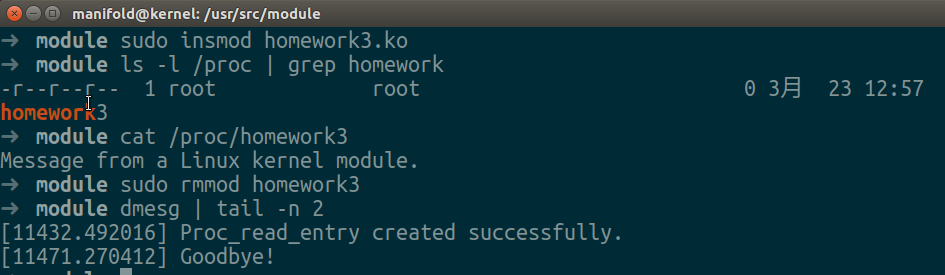
\includegraphics[width=12cm]{hw3.png}
\caption{Result of homework 3}
\end{figure}


\section{Conclusion}
This is the first project that we do real programming on Linux kernel. Linux kernel module is a very important part of kernel programming and I think during this project I really learned a lot about kernel module development and \texttt{/proc} file system. Also, finding information from various documentations is a very important skill for computer science students since many system projects are so large that we have to refer to docs to know what is actually happening and Linux kernel is no exception.


\section*{Acknowledgement}
Thanks Prof. Chen for guidance on Linux kernel and TAs for their hard work.
\end{document}
